\clearpage
\section{Praktischer Selbstversuch}
\label{sec:practice}

Um die Schlussfolgerungen aus dem Forschungsteil weiter zu untersuchen, wurde entschieden, die Vor- und Nachteile der Lerntypen in einem praktischen Selbstversuch zu betrachten.
Es soll hierbei speziell untersucht werden, welche Schwierigkeiten erwartet werden, und welche tatsächlich bei der Bearbeitung auftreten.
Hierzu werden die einzelnen Lerndimensionen der Autorin untersucht. Anschließend wird ein einfacher Algorithmus in einer funktionalen Programmiersprache umgesetzt. Es wurde sich für Haskell entschieden, da es die meistverwendete funktionale Programmiersprache in Einsteigerkursen im Bereich Informatik ist (siehe \nameref{sec:curriculares}).
Zur Vorbereitung wurde der Kurs CIS 194 \cite{cis194} der University of Pennsylvania genutzt, der in der offiziellen Haskell-Dokumentation empfohlen wird \cite{haskelldoc}.
Als Problem wurde "Türme von Hanoi" gewählt. Weitere Erläuterungen zu der Art des Problems folgen in Abschnitt \nameref{sec:problemdesc}.

\subsection{Lerntypenanalyse}
Um den Selbstversuch mit den Vor- und Nachteilen der Lerntypen zu verbinden, musste zunächst eine eigene Lerntypenanalyse durchgeführt werden.
Hierzu wurde der "Index of Learning Styles Questionnaire" verwendet \cite{ils_questionnaire}, ein Online-Tool, welches insgesamt 44 Fragen stellt und dann auf Basis der Antworten die Lerntypen eines Individuums einschätzen kann. Die Lerntypen werden als Gegensatzpaare auf einer Skala gezeigt, die darstellen soll, wie ausgeprägt der Hang zu einem Aspekt ist. Ein Wert von 1 bis 3 entspricht einer ausgewogenen Balance beider Aspekte der Dimension, 5 bis 7 entspricht einem mäßigen Hang zu einem Aspekt und 9 bis 11 entspricht einer starken Präferenz für einen der Lernstile.
Die Verlässlichkeit dieses Fragebogens wurde sowohl von den ursprünglichen Autorinnen des Lernmodells \cite{felder2005} als auch von anderen Quellen \cite{zywno} geprüft und bestätigt.

\subsubsection{Ergebnisse der persönlichen Evaluierung}
Die Fragen des ILS Fragebogens wurden in einer zufälligen Reihenfolge beantwortet, um zu vermeiden, dass bereits vorab klar ist, welche Frage welcher Typendimension zugeordnet ist. Dies ist möglich, da der Test so aufgebaut ist, dass jeweils ein Frageblock von 4 Fragen jede Dimension behandelt. Die erste Frage beispielsweise fließt in die Bewertung der aktiv/reflexiven Dimension ein, ebenso wie die fünfte und neunte Frage.

Die Ergebnisse des Fragebogens lauten wie folgt.

\begin{figure}[H]
    \centering
    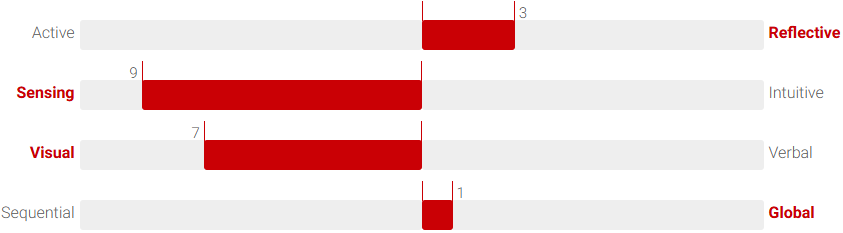
\includegraphics[width=1\linewidth]{Figures/Section_4/ILS_result}
    \caption{Ergebnisse des ILS Fragebogens}
\end{figure}

Die Autorin zeigt demnach folgende Ausprägungen in den Dimensionen.

\begin{itemize}
    \item Ein ausgewogenes Verhältnis der aktiven/reflexiven Dimension
    \item Eine starke Präferenz für den sensorischen Typ
    \item Eine mäßige Präferenz für den visuellen Typ
    \item Ein ausgewogenes Verhältnis der sequenziellen/globalen Dimension
\end{itemize}

Die individuellen Ausprägungen der Lerntypen werden im praktischen Versuch hinsichtlich des Erlernens und Anwendens der CT Aspekte und der verschiedenen Paradigmen untersucht.
Die Ausprägungen sollten sich demnach wie folgt auswirken.

\begin{itemize}
    \item Kein besonderer Vor- oder Nachteil beim Debugging in funktionaler Programmierung (FP), und beim Erlernen von Programmieren in Einzelarbeit
    \item Ein Nachteil beim Anwenden von algorithmischem Denken und der Erkennung der Zusammenhänge zwischen FP und mathematischen Funktionen, sowie beim innovativen Arbeiten mit einem limitierten Toolset
    \item Ein möglicher mäßiger Vorteil bei der Dekomposition aus der Perspektive eines visuellen Lerntypen, sowie zur Abstraktion auf Funktionsebene in der FP
    \item Kein besonderer zusätzlicher Vorteil bei der Dekomposition aus der Perspektive eines sequenziellen Lerntyps, sowie der generellen Anwendung von FP in einer sequenziellen Lösungsstrategie
\end{itemize}

\subsection{Problembeschreibung}\label{sec:problemdesc}
Um die aufgestellten Thesen zu prüfen, wurde entschieden, eine Programmieraufgabe in einem praktischen Teil zu lösen und alle Erfahrungen, Schwierigkeiten und Probleme in einer Art "Development Diary" zu dokumentieren.
Als Problem für den praktischen Versuch wurden die "Türme von Hanoi" gewählt. Diese Entscheidung wurde getroffen, da die Aufgabe in einem Anfängerkurs mit eigener Aufgabenstellung vertreten war \cite{cis194}, sowie alle Aspekte des CT abdeckt. Das Problem erfordert zudem die Anwendung von Rekursion, was in der FP einen besonderen Stellenwert hat.
Die Aufgabenstellung des Kurses CIS 194 bietet einen Ansatz in Form einer vorgegebenen Funktionsdefinition, sowie zwei vordefinierten Datentypen. Aufgrund dessen, dass auch der Aspekt der Abstraktion und Dekomposition betrachtet werden sollte, wurde die Aufgabenstellung des Kurses CIS 194 nicht verwendet. Stattdessen wurde von Grund auf selbst eine Lösung gefunden.

In dem Problem geht es um drei Holzstäbe, auf denen unterschiedlich große, runde Holzplatten gestapelt sind. Das Ziel der Lösung ist es, die aufsteigend gestapelten Platten vom Turm ganz links hin zum Turm ganz rechts zu transportieren. Hierbei gelten drei Regeln. Zum einen darf nie mehr als eine Platte gleichzeitig bewegt werden. Eine Platte darf nur bewegt werden, wenn diese die oberste im Stapel ist. Außerdem darf sich eine größere Platte niemals auf einer kleineren befinden.

\begin{figure}[H]
    \centering
    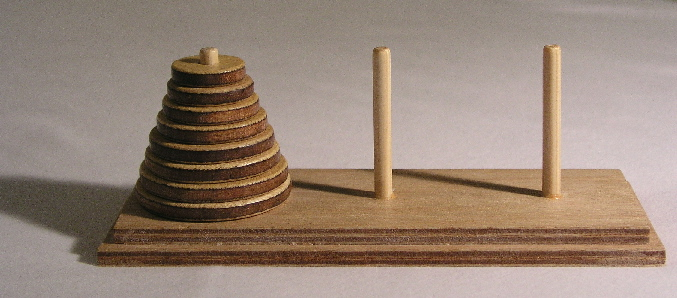
\includegraphics[width=1\linewidth]{Figures/Section_4/hanoi}
    \caption{Ein Modellset der Türme von Hanoi mit 8 Holzplatten \protect\cite{wikicommons}}
\end{figure}

\subsubsection{Theoretische Überlegungen}
Um das Problem zu lösen, wurde zunächst unabhängig vom Code über das Problem nachgedacht. Da ein mäßiger Hang zum visuellen Lerntypen besteht, wurde entschieden, das Problem physisch nachzubauen. Diese Methode half besonders dabei, das Problem zu verstehen und erste Überlegungen zur Abstraktion des Problems durchzuführen. Zunächst wurde versucht, durch zufälliges Ausprobieren eine Lösung zu finden. Dies funktionierte, allerdings wurden keine besonderen Muster gefunden, die bei einer allgemeinen Lösung des Problems helfen könnten.

Die ersten tatsächlichen Lösungsansätze waren sehr kompliziert, da noch kein globales Verständnis für das Problem vorhanden war. Zunächst wurde überlegt, wie das Problem abstrahiert werden kann.
Die Holzplatten wurden hierbei als Integer abstrahiert, um einfach die Größen vergleichen zu können. Die Pole selbst wurden als Listen dargestellt, in denen jeweils das erste Element (der "Head" der Liste) die oberste Holzplatte darstellt.
Ob eine Bewegung dem legalen Bewegungsset entspricht, wird anhand dessen bestimmt, ob das zu bewegende Element kleiner ist, als das Element, auf dem dieses platziert wird. Elemente werden dann so lange bewegt, bis die "Win Condition" erreicht ist, in dem Fall, dass sich in den ersten beiden Listen keine Elemente mehr befinden.
Es wurde allerdings schnell bemerkt, insbesondere beim Durchspielen des Ansatzes am physischen Modell, dass sich schnell Endlosschleifen entwickeln. Um einen neuen Ansatz zu finden, wurde deshalb auf Online-Visualisierungen zurückgegriffen.

Das Problem wurde zunächst in der simpelsten Form betrachtet, mit insgesamt drei Holzplatten. Es zeigte sich, dass es das erste "Teilziel" des Problems ist, die größte Platte auf den rechten Pol zu setzen. Die anderen Platten werden durch Hilfsschritte geordnet und in der Mitte als Hilfspol zwischengelagert. Dieser Ansatz half stark dabei, Muster in der Lösung zu erkennen.

Erst an diesem Punkt wurde klar, wie das Problem rekursiv gelöst werden kann. Falls mehr als 3 Holzplatten vorhanden sind, kann das Problem so lange weiter reduziert werden, bis nur noch drei Platten betrachtet werden. Von dort aus lässt sich das Problem rekursiv mit n-1 Platten lösen.

\subsubsection{Abstraktion}

Da die Funktion rekursiv laufen soll, muss sie alle nötigen Parameter entgegennehmen. Hierzu gehören der Startpol, Zielpol, und gegebenenfalls ein Hilfspol, auf dem Platten zwischen platziert werden können. Zudem wird die Anzahl von Holzplatten benötigt, die sich in jedem rekursiven Schritt reduziert. Die Pole selbst werden als Listen von Integern modelliert.
Um die Schritte zur Lösung zu dokumentieren, wird zudem eine Liste von Lösungsschritten übergeben, die jeweils in einem Tupel den Startpol sowie den Endpol dokumentiert. Diese Liste von Lösungsschritten repräsentiert letztendlich die finale Lösung und ist eine Anleitung zur Problemlösung.

Im Problem lassen sich nur wenige Teilverantwortlichkeiten identifizieren, da der größte Teil der Arbeit im rekursiven Schritt liegt. Allerdings lässt sich im Vergleich zu herkömmlichen, nicht funktionalen Lösungen sagen, dass das Erstellen und Füllen der Liste mit Lösungsschritten ein zusätzlicher Aspekt ist, der in der Lösung berücksichtigt werden muss. Die Schritte können zum Beispiel nicht während der Berechnung kontinuierlich in der Konsole gedruckt werden, da Funktionen in der FP keine Seiteneffekte zulassen.

\subsection{Umsetzung}

Die Umsetzung des Problems im funktionalen Paradigma erfolgte in Haskell. % WIP

\subsection{Zusammenhang mit Lerntypen}
Beim Bearbeiten der Aufgabe wurden einige Beobachtungen speziell im Zusammenhang mit der Forschung aus Abschnitt 3 der Arbeit gemacht. Es wurde erwartet, dass besonders die Dekomposition und Abstraktion leichter fallen, allerdings Schwierigkeiten beim Finden der Algorithmik und der Zusammenhänge der Teilprobleme auftreten.

Die Beobachtungen aus dem praktischen Versuch stützen diese Annahmen. Der Prozess der theoretischen Lösungsfindung, das Aufteilen des Problems in Teilprobleme, sowie die Abstraktionsphase waren alle Aspekte, die relativ einfach waren. Die Schwierigkeiten traten in der Findung des tatsächlichen Algorithmus, sowie dem Erkennen des globalen Zusammenhanges auf. Besonders traten diese Probleme in der Phase der Musterfindung auf, speziell bei der Frage, wie man den Algorithmus allgemeiner und rekursiv gestalten kann.
